\lab{Application}{Depth and Breadth First Search with Kevin Bacon}{Depth and Breadth First Search with Kevin Bacon}
\label{lab:SixDegreesKevinBacon}

\objective{This section teaches about searching graphs and uses the parlor game ``Six Degrees of Kevin Bacon'' as an application to graphs.}

\section*{Graphs}
Graphs are often used to represent relationships between objects. They are
represented by a set of nodes (or vertices) and a set of edges where each edge
connects exactly two nodes. We would indicate an edge from node $A$ to node $B$ by $(A, B)$
and an edge from $B$ to $A$ by $(B,A)$. If \emph{all} of the edges within the graph are bidirectional
between their connecting nodes, the graph is said to be \emph{undirected}. If, however, the directions
of the graph's edges are specified, then the graph is said to be \emph{directed}. In this lab, however, we will largely be working
with undirected graphs.

There are two different data structures that can be used to represent graphs: adjacency matrices and adjacency lists.
Each data structure has its own advantages and disadvantages;
which one you use mostly depends on the type of problem you are solving.
\begin{comment}
\begin{figure}[h]
\centering
\includegraphics[width=.5\textwidth]{adjacency_example_graph.pdf}
\caption{An example graph.}
\label{fig:bfs_dfs_graph}
\end{figure}
\end{comment}
\subsection*{Adjacency Matrices}
An Adjacency matrix is two dimensional matrix used to represent a graph. We order
the nodes of the graph and allow each node to correspond to one column and one
row of the matrix. Therefore, if we have $n$ nodes, we use an $n \times n$ matrix to
represent the edges between the nodes. In an unweighted graph (a graph where all the edges have the same value), we indicate an
edge between two nodes using either a 0 or a 1.
Consider the example graph in Figure 4.1. Because a bidirectional edge exists between A and D, for example, we put a 1 in the (4,1) position and
in the (1,4) position. Since no edge exists between A and C, we put a 0 in
the (3,1) position and (1,3) position. We can represent the adjacency matrix for this graph as follows:

\[
\bordermatrix{\hspace{.4cm}&A&B&C&D&E\cr
                A&0 & 1 & 1 & 0 & 1\cr
                B& 1 & 0 & 0 & 1 & 0\cr
                C& 1 & 0 & 0 & 0 & 0\cr
                D& 0 & 1 & 0 & 0 & 1\cr
                E& 1 & 0 & 0 & 1 & 0}\]
Note that because this graph is undirected, its adjacency matrix is symmetric. 

\begin{comment}
If a graph has $n$ nodes, then representing it as an adjacency matrix requires a $n \times n$ matrix. Each node corresponds to the same row and column number.
The $ij$th entry of the adjacency matrix represents the edge between nodes associated with row $i$ and column $j$.
If the entry is 0, then no edge exists between nodes $i$ and $j$, otherwise there is is an edge between nodes $i$ and $j$.
An adjacency matrix allows us to query the existence of an edge, or its edge weight, in constant time.
\end{comment}
\subsection*{Adjacency Lists}
An adjacency list links each node of the graph to a list of its corresponding neighbors, the nodes to which it is connected by an edge.
There are many ways to index the nodes so their \emph{adjacent} neighbors can be easily queried, but one of the most straightforward ways in Python is to use a simple dictionary. 
We might represent our example graph using the following code:
\begin{lstlisting}
AList = {'A': ['B', 'D', 'E'], 'B':['A', 'C'], 'C':['B', 'D'], 'D':['A', 'C'], 'E':['A']}
# To obtain a list of the nodes adjacent to A, simply access the
# dictionary at the key 'A'.
print Alist['A']
# You should obtain the following output:
['B', 'D', 'E']
\end{lstlisting}
We can query the neighbors of any node in the graph in constant time.
This makes algorithms that operate locally on the graph very efficient.

\section*{Searching Graphs}
There are two common ways to search a graph, both of which present different advantages depending on the purpose of the search.
One method is called a depth-first search (DFS).  It is designed to search the deepest levels of a graph first.
The other method is called a breadth-first search (BFS).  BFS searches the graph one level at a time until it finds a solution.
\begin{figure}[h]
\centering
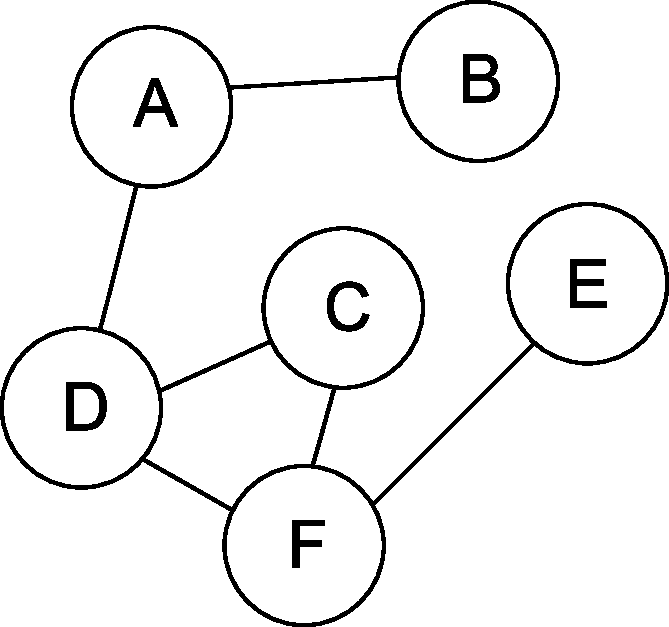
\includegraphics[width=.5\textwidth]{graph.pdf}
\caption{An example graph.}
\label{fig:bfs_dfs_graph}
\end{figure}


Here, we will walk through two examples of a depth-first search.
In these examples, when a node has multiple branches originating from it,
we will visit the latest (greater) letter in the alphabet first.
We call the node at which the algorithm begins the ``root node''.
First, we will use D as our root node and E as our target node.
Starting at D, we look at its greatest neighbor, F, then at F's greatest
neighbor, E. Since E is our target, the algorithm ends.

Second, we will start with A and search for B.
We visit node A, then D, then F, and finally, E.
At this point, we have gone as deeply as we can and have still not found our target, B.
We must then back up and try another branch of nodes.
The algorithm backtracks from E to F and tries another route.
Since we have marked D as previously visited, we visit F's final neighbor, C.
Note that it is very important that we mark those nodes we have already visited,
otherwise the algorithm would infinitely loop around the latter portion of
the graph without reaching our target, B. We return to node F. Since we have
searched all possible nodes adjacent to F, we backtrack, again, to D. Because we have
exhausted all sub-branches originating from D, we travel back to A and try
any unexplored branches there. Finally, we find B and the algorithm ends.

Let's try the same two searches using a breadth-first search. This time, however,
we will visit the earliest (lesser) letter in the alphabet first while
exploring our branches. In this first search, we again use D as our root node and
E as our target node.
We start by searching for E among the neighbors of D: A, C, and F.
We have not found E, so we search among the neighbors of these adjacent nodes, starting with A.
B is the only neighbor of A that we have not already visited; we backtrack to our previous collection of neighbors: A, C, and F.
We have already visited both neighbors of C (D and F), so we continue to the adjacent nodes of F. Finally, we find E among the neighbors of F, and the algorithm ends.

In the second search, we start with A.
Since B is a neighbor of A, we find it immediately.

Both DFS and BFS have advantages.
If we are able to choose a root node that is local to the target node, BFS is obviously the better choice. However,
DFS can be much more efficient when the solution is far from the target node.
Algorithm \ref{alg:BFSDFS} outlines the process by which we may implement BFS and DFS methods, respectively.
\begin{comment}

\end{comment}

\begin{algorithm}
\begin{algorithmic}[1]
\Procedure{BFS/DFS}{$G, root, destination$}
	\State $Q \gets \text{Deque (BFS) or list (DFS) with root node in it}$	\Comment{Initialization steps}
	\State $marked \gets \text{Set with root node in it}$	
	\State $visited \gets \text{empty list}$	
	\While{$Q \text{ has elements}$}						\Comment{Go through the graph.}
		\State $t \gets Q\text{'s left (BFS) or right (DFS) element}$	
		\State $\text{add }t \text{ to the visited list}$
		\If{$t==destination$}							\Comment{Found the destination node.}
			\State \pseudoli{return} $t,visited$
		
		\Else										\Comment{Visit $t$'s neighbors.}
			\For{$k \text{ in the adjacent nodes of } t$}
				\If{$k \text{ not in } marked$}
					\State $\text{add } k \text{ to } marked$
					\State $\text{add } k \text{ to } Q$
				\EndIf
			\EndFor
		\EndIf
	\EndWhile
\EndProcedure
\end{algorithmic}
\caption{Breadth-first and depth-first search}
\label{alg:BFSDFS}
\end{algorithm}

\begin{problem}
Implement methods that will perform depth-first and breadth-first searches on a graph (in this case, an adjacency list).
Use a \li{set()} to store the visited nodes. (Because Python implements sets as hash tables, they have very efficient membership testing.)

\emph{Helpful Hint}: The implementations of a depth and a breadth first search
are almost exactly same, but they use a particular data structure differently.
\begin{itemize}
\item Which data structure constitutes this important difference?
\item How is it used differently?
\end{itemize}
\end{problem}

\section*{Bidirectional Searching an Unweighted Graph}
\begin{comment}
\begin{figure}[h]
\centering
\includegraphics[width=.75\textwidth]{Bidirectional.pdf}
\caption{An example graph.}
\label{fig:bfs_dfs_graph}
\end{figure}
\end{comment}
Let A be an unweighted graph. This means that none of the edges of A has any value, or ``weight'' attached to it. How can we find the shortest path between two nodes?
One way would be to simply use a breadth first search, stopping when we reach the target node. The downside to doing it this way is that the algorithm would look through (at least)
every node on every level prior to the target node before it could end. Observe the example graph above. Let us use a simple BFS to search for O, starting with A as our root node.
We then search through all of the neighbors of A, all of the neighbors of B and C, and so on until we finally locate O. Using this method, we are forced to check
a total of $15$ nodes before our algorithm ends.

A better way to find the shortest path is to do a breadth-first search from both A and O. Thus, we find the shortest path between A and O using a pair of breadth-first searches originating from the root node and target node, respectively.
We advance each BFS one node at a time, alternating until they meet, and then construct the shortest path of nodes between them.
 Using our BFS algorithm from above, we start with A and locate its
least neighbor, B. Since we have not yet found O (or a connection to O) we visit G, the first neighbor of O. Continuing in this pattern, we return to the neighbors
of A to visit C. We return to our second search to visit the least neighbor of G, which is also C. We have found our connection, so the algorithm ends. Note that when we used a breadth first
searched with only one root node, we visited $15$ nodes, but when we used a bidirectional BFS, we only had to visit a total of $5$ nodes to reach our target.

When you have many more nodes each level away, the speedup from doing a breadth-first search from both sides is far greater. This is one of the best ways to find shortest
paths in unweighted, undirected graphs. For weighted graphs there are many algorithms that allow us to find the shortest path. For further information research
the Bellman–Ford algorithm,the Floyd–Warshall algorithm, Johnson's algorithm, Dijkstra's algorithm, and A* search algorithm.

\section*{Six Degrees of Kevin Bacon}
\begin{figure}[h]
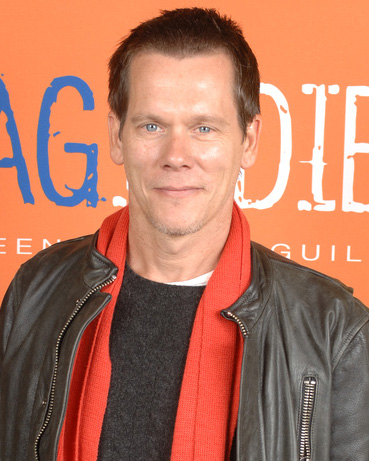
\includegraphics[scale = .4]{Kevin_Bacon.jpg}
\caption{Kevin Bacon.  Image source: Wikipedia.}
\end{figure}

The theory of ``the 6 Degrees of Separation'' suggests that each person in the world can be linked to any other person by 6 or less steps of acquaintanceship.
Similarly, the game ``6 Degrees of Kevin Bacon'' contends that every actor in the film industry can be linked to Kevin Bacon by 6 degrees or less. Kevin Bacon
is a prolific American actor whose film career spans over 30 years in a variety of genres. As such, he once reputably commented that he had either worked with everyone in
Hollywood or someone who has worked with them. The goal of the game, then, is to find the lowest Bacon number for each actor, a process demonstrated as follows:
\begin{enumerate}
\item Kevin Bacon has a Bacon number of 0.
\item Actors that have been in a movie with Kevin Bacon have a Bacon number of 1.
\item For all other actors $X$, if the lowest number of any actor that $X$ has been in a film with is $n$, $X$ has a Bacon number of $n+1$.
\end{enumerate}

\begin{figure}[h]

\includegraphics[scale = .6]{Example}
\caption{Jeffery Humphery was in \emph{End Game} with Cuba Gooding Jr. who was in \emph{A Few Good Men} with Kevin Bacon, so Jeffrey Humphrey has a Bacon Number of 2.  Image source: http://oracleofbacon.org/.}
\end{figure}

You can define a graph in the same way: where each actor is a node and there is an edge between any two nodes if the actors were in a movie together. From this structure you can find
the shortest path between any actor and Kevin Bacon by using any of the algorithms listed above. Of course, we could play this game with any actor as our ``root actor'' rather than Kevin Bacon. In
fact, ``the Six Degrees of Separation'' can be applied to many different fields. The most famous of its applications is known as the Erdos numbers: how far away is a person
 from publishing a paper (rather than starring in a movie) with the prolific mathematician Paul Erdos?

\section*{NetworkX}
For this lab, we are going to use a network library called NetworkX. NetworkX is a useful Python package that allows us to create and manipulate large, complex networks.
When considering efficiency, however, it is important to note that because NetworkX uses Python objects to represent its graphs internally, graphs with many nodes will
take a large chunk of memory. (Other network libraries, such as igraph, are written in C++ and may therefore significantly reduce the overhead of storing such a graph.)
To make an undirected graph in NetworkX you code the following:

\begin{lstlisting}
import networkx as nx
G = nx.Graph()
\end{lstlisting}

As an example, we will create a NetworkX graph that links the ingredients of delicious Italian foods together. We first want to add the ingredients as nodes to our graph.
To add nodes we can use the \li{add_node(x)} method where $x$ is the node we want to add or we can use the \li{add_nodes_from} method to add multiple nodes at once.

\begin{lstlisting}
import networkx as nx
G = nx.Graph()

G.add_node('dough')
PizzaIngredients = ['dough','mozzarella cheese','tomato sauce','ham','pineapple']
G.add_nodes_from(PizzaIngredients)
\end{lstlisting}
Note that even though we added \li{'dough'} twice, the graph will only store this node once. NetworkX also comes with \li{has_node(x)} and \li{has_edge(x,y)} methods that tell
us if the node \li{x} or edge \li{x,y} has already been added.

Now we want to connect our pizza ingredients together. Adding an edge is simple; we use the \li{add_edge(x,y)} method, where $x$ and $y$ are previously added nodes.
Again, we can also add multiple edges using the \li{add_edges_from()} method. However, these edges must be provided as 2-tuples (u,v), so we use the itertools module to create a list of the edges we want to add.

\begin{lstlisting}
from itertools import permutations
Pizza = permutations(PizzaIngredients, 2)
G.add_edges_from(Pizza)
\end{lstlisting}
If you add an edge between two non-existent nodes, the missing nodes will also be added to the graph. Let's add the ingredients for lasagna to the graph using only the \li{add_edges_from} method.
\begin{lstlisting}
LasagnaIngredients = ['lasagna noodles','sausage','mozzarella cheese','cottage cheese','tomato sauce','egg','parsley']
Lasagna = permutations(LasagnaIngredients, 2)
G.add_edges_from(Lasagna)
\end{lstlisting}
We can also remove nodes using the \li{remove_node(x)} and \li{remove_nodes_from()} methods respectively. Let's say, for example, that we are vegetarians and want to remove the sausage and ham from our graph. Then, we simply run the following code:
\begin{lstlisting}
G.remove_nodes_from(('sausage','ham'))
\end{lstlisting}

Sometimes, with smaller graphs, it can be useful to visualize how nodes are linked together. However, the overhead associated with displaying larger graphs makes this unwise for extensive data sets.
For our example, though, it is easy to see the connections between our lasagna and pizza ingredients:

\begin{lstlisting}
# MatPlotLib is a standard plotting library, it allows you to plot
# and display your 2D graph.
import matplotlib.pyplot as plt
# Allows you to draw a simple diagram of the nodes and their connecting edges.
nx.draw(G)
# Displays your graph.
plt.show()
\end{lstlisting}


\begin{problem}
The data file, \texttt{movieData.txt}, contains the entire casts of movies made from 2011 to August of 2013. It is a delimited file with each field delimited by the '/' character. Write a method that will implement the following:
\begin{itemize}
\item Open the file.
\item Generate a NetworkX graph, with the actors as nodes and with edges connecting all of the actors within the same movie. Do not include movie titles as nodes.
\item Return your constructed NetworkX graph (note that, because of the large amount of data, you \textbf{should not} attempt to display this graph).
\end{itemize}
\emph{Helpful Hints:}
\begin{itemize}
\item For later solutions, it might be beneficial to also construct a map from actors to the movies that they appeared in.
\item When opening your file with a Window's machine, take care to use universal newline support. See Lab 1 for further information.
\end{itemize}
\end{problem}

The \li{shortest_path(G, x, y)} function in NetworkX outputs a list that is one of the shortest paths between $x$ and $y$ in graph $G$.  In an unweighted graph, it finds 
the shortest path using a bidirectional search, as outlined earlier in this chapter. If no target is specified, the function will find the shortest paths between $x$ and every 
other node in the network.  It will return the results in a dictionary.  If more than one ``shortest path'' exists, it will return the first one it finds.  We can find the 
length of the shortest path using the \li{shortest_path_length(G, x, y)} function.

\begin{problem}
Find the shortest path between Kevin Bacon and Liam Neeson. Then find the shortest path from Kevin Bacon to Imran Zahid. Write a function that will accept a path and output 
the path with the movies in between that connect the actors. Output the paths from Kevin Bacon to Liam Neeson and Imran Zahid with the connecting movies.
\end{problem}

\begin{problem}
Find the average Bacon number for the dataset. Then find how many people have each Bacon number and how many people are not connected to Kevin Bacon at all (these people have 
a Bacon number of infinity).
\end{problem}

